\section{Newtons 2. lov og bevægelsesligninger} \label{mek:sec:fjeder}
Hovedformålet med klassisk mekanik er at undersøge systemer i vores verden, specifikt at kunne beskrive bevægelser, som vi ser dem.
Newtons love, specielt hans 2. lov\footnote{Her er den skrevet på vektorform, der betyder, at den gælder for hvert koordinat i det koordinatsystem, man vælger at benytte.},
%
\begin{align} \label{mek:eq:N2}
	\sum\va{F} = m\va{a} = m\dv[2]{\va{r}}{t},
\end{align}
%
lægger den grundlæggende byggesten for, hvordan klassiske mekanik beskrives. Beskrevet med ord siger \cref{mek:eq:N2}, at summen af alle kræfter på et legeme, er det samme som legemets masse gange legemets acceleration. I \cref{mat:ex:diff_lign} så vi hvordan Newtons anden lov kan bruges til at opstille bevægelsesligninger. De fleste differentialligning, man støder på i fysik, er af anden orden. Derfor kigges nu på et sådan eksempel, nemlig en klods på en fjeder.
% Hvordan bruger man det til vores formål, nemlig at kunne beskrive objekters bevægelse? For at svare på dette tages udgangspunkt i kraftanalyse og et eksempel med et lod på en fjeder.

\begin{figure}[]
	\centering
	%
	\begin{tikzpicture}[line width=2pt]
	    \draw (-1,3) to (-1,0) to (9,0);
	    \draw (3,0) to (6,0) to (6,2) to (3,2) to (3,0);
	    %
	    \fill [pattern = north east lines] (-1,-.5) rectangle (9,0);
	    \fill [pattern = north east lines] (-1,-.5) rectangle (-1.5,3);
	    %
	    \draw[decoration={aspect=0.5, segment length=3mm, amplitude=3mm,coil},decorate] (2.75,1) -- (-0.85,1);
	    \draw (-1,1) to (-0.85,1);
	    \draw (2.75,1) to (3,1);
	    %
	    \draw[-{Stealth[length=5mm, width=3mm]}] (4.5,1) to (7.5,1);
	    %
	    \draw (6.75,1.15) node[anchor=south]{\LARGE $\va{F}_\textup{fj}$};
	    \draw (1,1.4) node[anchor=south]{\LARGE $k$};
	    %
	    \draw[-{Stealth[length=4mm, width=2.5mm]}] (8,2) to (9,2);
	    \draw[-{Stealth[length=4mm, width=2.5mm]}] (8,2) to (8,3);
	    %
	    \draw (8.3,2) node[anchor=north]{\LARGE $\vu{x}$};
	    \draw (7.7,2.65) node[anchor=north]{\LARGE $\vu{y}$};
	\end{tikzpicture}
	%
% 	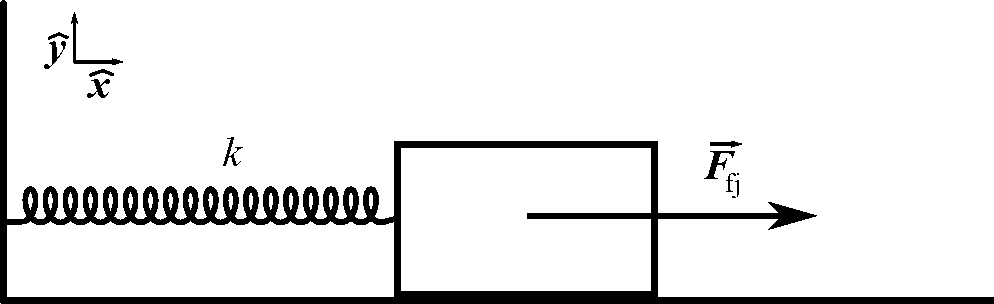
\includegraphics[width=.75\textwidth]{figurer/Fjeder.pdf}
	\caption{En klods med massen $m$, der er fastspændt på en fjeder med fjederkonstant $k$, hvor det hele er på en friktionsløs overflade. På tegningen er fjederen sammenpresset, hvorfor fjederen påvirker klodsen med en kraft, $\va{F}_\textup{fj}$, i den viste retning. Enhedsvektorerne i øverste højre hjørne viser at $x$-aksen er vandret, og $y$-aksen er lodret.} \label{mek:fig:fjeder}
\end{figure}
%
\begin{example}[Klods på en fjeder] \label{mek:ex:ho}%
På \cref{mek:fig:fjeder} ses en illustration af en fjeder fastspændt på en klods, hvor overfladen, som klodsen bevæger sig på, er friktionsløs. Fjederen har fjederkonstanten $k$ og klodsen har massen $m$. Her ses bort fra alle former for friktion, hvilket betyder at fjederkraften er den eneste kraft, der virker på klodsen. Inden man kaster sig ud i matematikken, er det værd at overveje hvilken løsning, man forventer at få. Når fjederen er presset sammen, vil den forsøge at udvide sig, og når den er udstrakt, vil den forsøge at trække sig sammen. Det betyder, at klodsen svinger frem og tilbage omkring et ligevægtspunkt. Det forventes at bevægelsen er periodisk -- det vil sige at bevægelsen gentager sig. Her defineres koordinatsystemet således at klodsen i sin hvileposition er i $x = 0$, hvorved klodsens bevægelse kan beskrives med en sinus- eller cosinusfunktion. Her vælges cosinus\footnote{Havde man valgt sinus, ville det bare ændre værdien af $\delta$ med $\pi/2$. Pr. konvention vælges ofte cosinus, hvorfor det samme gøres her.} på formen
%
\begin{align} \label{mek:eq:FjederSted}
	x(t) = A\cos(\omega t + \delta),
\end{align}
%
hvor $t$ er tiden, mens $A$, $\omega$ og $\delta$ er konstanter. Cosinusfunktionen svinger mellem $-1$ og $1$, hvorfor $A$ er den maksimale afstand fra $x=0$, som klodsen kan have. $\omega$ er vinkelfrekvensen, der beskriver hvor hurtigt klodsen svinger frem og tilbage.
Fjederkonstanten $k$ er et udtryk for, hvor ``hård'' fjederen er, det vil sige hvor meget energi det kræver, at presse fjederen sammen, mens massen $m$ er et mål for, hvor meget energi der skal til, for at ændre klodsens bevægelse. En logisk forventning ville derfor være, hvis $\omega$ på en eller anden måde afhænger af $k/m$. $\delta$ er en faseforskydningskonstant, og dens betydning ses ved at kigge på funktionen til tiden $t=0$. Her bliver $x(0) = A\cos\delta$, hvorfor $\delta$ beskriver hvor lodet er i sin bevægelse til tiden $t=0$. Cosinus er en periodisk funktion, der svinger frem og tilbage, hvorfor det giver mening at kunne beskrive klodsen på den måde.

At \cref{mek:eq:FjederSted} faktisk beskriver klodsen, er det nu tid til at vise. Klodsen er påvirket af en fjederkraft
%
\begin{align} \label{mek:eq:hooke}
    F_\textup{fj} = -kx,
\end{align}
%
som afhænger af fjederens forskydning fra dens ligevægtspunkt, hvilket kaldes Hookes lov (opkaldt efter Robert Hooke), og den resulterende bevægelse kaldes Hookesk. Det, at fjederkraften har den form, er der ingen dybere teoretisk grund for, men det skyldes at eksperimenter viser, at fjedre kan beskrives på den måde, hvis de ikke deformeres\footnote{Fjederkraften stiger jo mere der trækkes eller skubbes til fjederen, men trækker man for meget i fjereden, strækkes den så meget, at den holder op med at opføre sig som en fjeder. Her ses kun på tilfældet hvor $x$ ikke bliver så stor, at fjederen ødelægges.}. Det er antaget, at fjederkraften er den eneste i systemet, hvorfor Newtons 2. lov i 1 dimension giver at
%
\begin{align} \label{mek:eq:hooke_newton}
    -kx = ma.
\end{align}
%
Dette ses ved at indsætte \cref{mek:eq:hooke} på venstresiden af \cref{mek:eq:N2}. Accelerationen $a$ er netop positionen af klodsen differentieret 2 gange med hensyn til tiden, $a = \dv*[2]{x}{t}$, se \cref{mat:eq:acceleration} og teksten omkring. Differentieres et koordinat mht. tiden benyttes priknotationen, $\dot{x} = \dv*{x}{t}$ og for dobbeltafledt $\ddot{x}$, fremover, hvorfor $a = \ddot{x}$. Dette betyder, at \cref{mek:eq:hooke_newton} er en 2. ordens differentialligning, der relaterer variablen $x$ til dens dobbeltafledte $\ddot{x}$:
%
\begin{align} \label{mek:eq:FjederDiffLign}
	m\ddot{x} = -kx.
\end{align}
%
Det særlige ved Newtons 2. lov er, at den giver os mulighed for at opskrive de bevægelsesligninger (differentialligninger), som vi skal løse, for at kunne beskrive vores system. Differentialligninger kendes fra kapitlet om matematik, \cref{mat:sec:diffeq}, og det huskes at løsninger til differentialligninger er funktioner, i modsætningen til almindelige ligninger, hvis løsninger er tal.
% Det er dog en hel del simplere at vise, at en funktion er en løsning til en differentialligning, end at finde en generel løsningsform dertil. At et tal er en løsning til en almindelige ligning, kan eftervises ved at sætte tallet ind på den ubekendtes plads, og så eftervise at ligningen går op. Det samme kan gøres med differentialligninger, hvor det så er funktionen, der indsættes.
Det blev påstået at \cref{mek:eq:FjederSted} beskriver klodsen, og derfor kan man prøve at indsætte den i differentialligningen, \cref{mek:eq:FjederDiffLign}. For at gøre det skal den dobbelt tidsafledte bestemmes
%
\begin{align}
\begin{aligned}
	\ddot{x} &=\dv[2]{}{t} \Big( A\cos(\omega t +\delta) \Big) = \dv{}{t} \Big( -\omega A \sin(\omega t + \delta) \Big) = -\omega ^2 A \cos(\omega t + \delta ) = -\omega^2x.
\end{aligned}
\end{align}
%
Indsættes det i \cref{mek:eq:FjederDiffLign} fås
%
\begin{align}
\begin{aligned}
	m(-\omega^2x) &= -kx \\
	\implies \omega^2 &= \frac{k}{m}.
\end{aligned}
\end{align}
%
Her ses det, at \cref{mek:eq:FjederSted} opfylder \cref{mek:eq:FjederDiffLign}, hvis $\omega^2 = k/m$. Med et snakkeargument fandt vi frem til, at $\omega$ måtte afhænge af $k/m$, og den præcise afhængighed er her opnået. Dette illustrerer at alt information, om hvordan et system opfører sig, er indeholdt i de differentialligninger, der kan opskrives ud fra Newtons love. De mest almindelige differentialligninger med deres løsning står i \cref{mat:tab:diffligninger}.
% Det kræver bare lige at de kan løses, hvilket eksempelvis kan gøres som her, ved at have et kvalificeret bud og så prøve efter, om det rent faktisk er en løsning. Man kan i nogle tilfælde bruge integration til at løse differentialligninger, hvilket kaldes separation af de variable. Ellers må man slå løsninger op eller finde numeriske løsninger med en computer.\footnote{Numeriske løsninger findes ved at sætte en computer til at regne en masse punkter, ud fra differentialligningen, til at forudsige opførslen af et bestemt system. Dette gøres tit, hvis der ikke kan laves fornuftige approksimationer til et system, eller for at teste fornuftigheden af de approksimationer man har lavet.}
\end{example}

\label{mek:page:ho_approx}
Som fysiker er det vigtigt, at kunne danne sig en forventning om hvordan stedfunktionen for et system opfører sig uden at regne på det. Dette er hvad vi gjorde for at finde frem til \cref{mek:eq:FjederSted}, og det er noget, som kommer med erfaring. Det erfaringen bruges til, er at sammenligne med andre ting man kender. \Cref{mek:eq:FjederDiffLign} er meget vigtig i fysik og den kaldes en harmonisk oscillator. Det gør den, fordi den beskriver symmetriske svingninger omkring et ligevægtspunkt, hvilket også hedder en harmonisk svingning/oscillation. Når man som fysiker møder noget, der svinger frem og tilbage, forventer man at det minder om en klodsen på en fjeder, hvilket er et af de simple, kendte eksempler.

% Det kan måske virke lidt som spildt arbejde at benytte differentialligningerne, hvis man kan gætte sig til en funktion, der beskriver systemet. Det svarer lidt til, at det i nogle tilfælde er ganske praktisk, at kunne gætte sig til en løsning til en almindelig ligning, men den metode afhænger af, at man har et godt gæt. Derfor er det smart at have en metode til faktisk at løse problemet, uden at skulle gætte sig frem.

% Det skal vise sig fremadrettet at være en rigtig smart og sikker fremgangsmåde først og fremmest at finde differentialligningerne (eller nærmere bevægelsesligningerne) for ens system, hvis man ikke kender bevægelsesligningerne på forhånd. For hvis man kan finde bevægelsesligningerne, så er det eneste man mangler, nemlig at løse differentialligningen, hvor man ofte kan lave nogle simplificerende antagelser, hvis løsningen ikke er oplagt.